%!TEX root = main.tex 

\section{Workload Tracing } 
\label{sec:workload_const_replay} 

% We first present in this section how \sys accurately traces the training workloads for each rank in an ex-situ fashion using a single device, thereby addressing Challenge 1 (\cref{subsec:challenges}). 
% We also show how \sys composes the global timelines across devices using the per-rank workloads to faithfully re-construct the entire training process in \cref{subsec:workload_replay}.



% 1. per-rank workload tracing;
% 2. replay to recover global timelines

\subsection{Per-Rank Workload Tracing} 
\label{subsec:workload_const}

% Generally, ML frameworks support various parallelism in distributed training in the following way: (1) they initialize each rank (typically one rank per device) with its own sub-model based on the parallelism setting, and then (2) each rank builds its own execution graph to start actual training. 
% As discussed in \cref{sec:overview}, \sys turns the parallel initialization process into a sequential one during job deployment to achieve faithful workload tracing without requiring the full cluster.
% \noindent \textbf{Iterative submodel initialization.}

To launch a training job, the ML framework registers the global parallelism parameters (e.g. DP/TP/PP/EP groups) given by user into the so-called model parallelism unit (MPU), which maintains all states related to parallelisms for a given rank.
Then according to the MPU, each rank concurrently initializes its own part of the model that it needs to train for (Figure \ref{fig:profier} \textcircled{1}
), and starts training with an execution graph that is optimized for its submodel based on the hardware/software environment and user configurations. 

\sys extracts the per-rank execution graph in an ex-situ fashion by transforming the above parallel process into a sequential one (Figure \ref{fig:profier} \textcircled{2}
). 
Specifically, \sys hijacks all the calls to the original MPU and re-directs them to its own MPU, and registers the global parallelism parameters as usual.
\sys's MPU only manipulates the input arguments to the MPU when necessary; it does not change the original implementation to ensure correctness.
Then with a single device, in each iteration $i$, \sys uses this unique rank ID $i$ to initialize the corresponding submodel and execute one complete training step, so all information regarding the computation \ops, including their dependencies (including those w.r.t other ranks) and running times, can be profiled.
For MoE workloads, \sys provides an interface to control token distributions across experts.
To ensure execution isolation, \sys launches each simulated rank as a separate single-process \texttt{torchrun} job, mirroring real distributed execution. Thus, the GPU only needs to hold one rank's model shard and step-local states at a time, so the memory requirement follows the largest per-rank shard under the target parallel configuration rather than the aggregate memory of all ranks.
Within this isolated execution, \sys runs the actual compute path for the current rank and samples GPU memory online, capturing allocator-level dynamics such as activation allocation, reuse, and early deallocation. Our current validation therefore focuses on per-rank training-step memory behavior excluding communication-time execution (see~\cref{subsec:workload_perf}).


The caveat here is collective communication: one device obviously cannot execute a communication \op. 
To resolve this, notice that when the communication \op is launched it also needs to call into the MPU which determines the device's position in the global communication groups for proper execution.
This is re-directed to \sys's MPU again allowing it to trace the communication \op's truthful information in the simulated setting (group association, message sizes, etc.); meanwhile, instead of returning results using the simulated (distributed) setting, \sys's MPU returns results corresponding to single device setting, so the communication \op can proceed and training is not blocked. 
This way \sys traces the actual execution graphs for each rank and running times of computation \ops without requiring the full-scale cluster.
Implementation details of tracing vary across frameworks which we will discuss in \cref{sec:implementation}.

\begin{figure}[t] 
    \centering 
    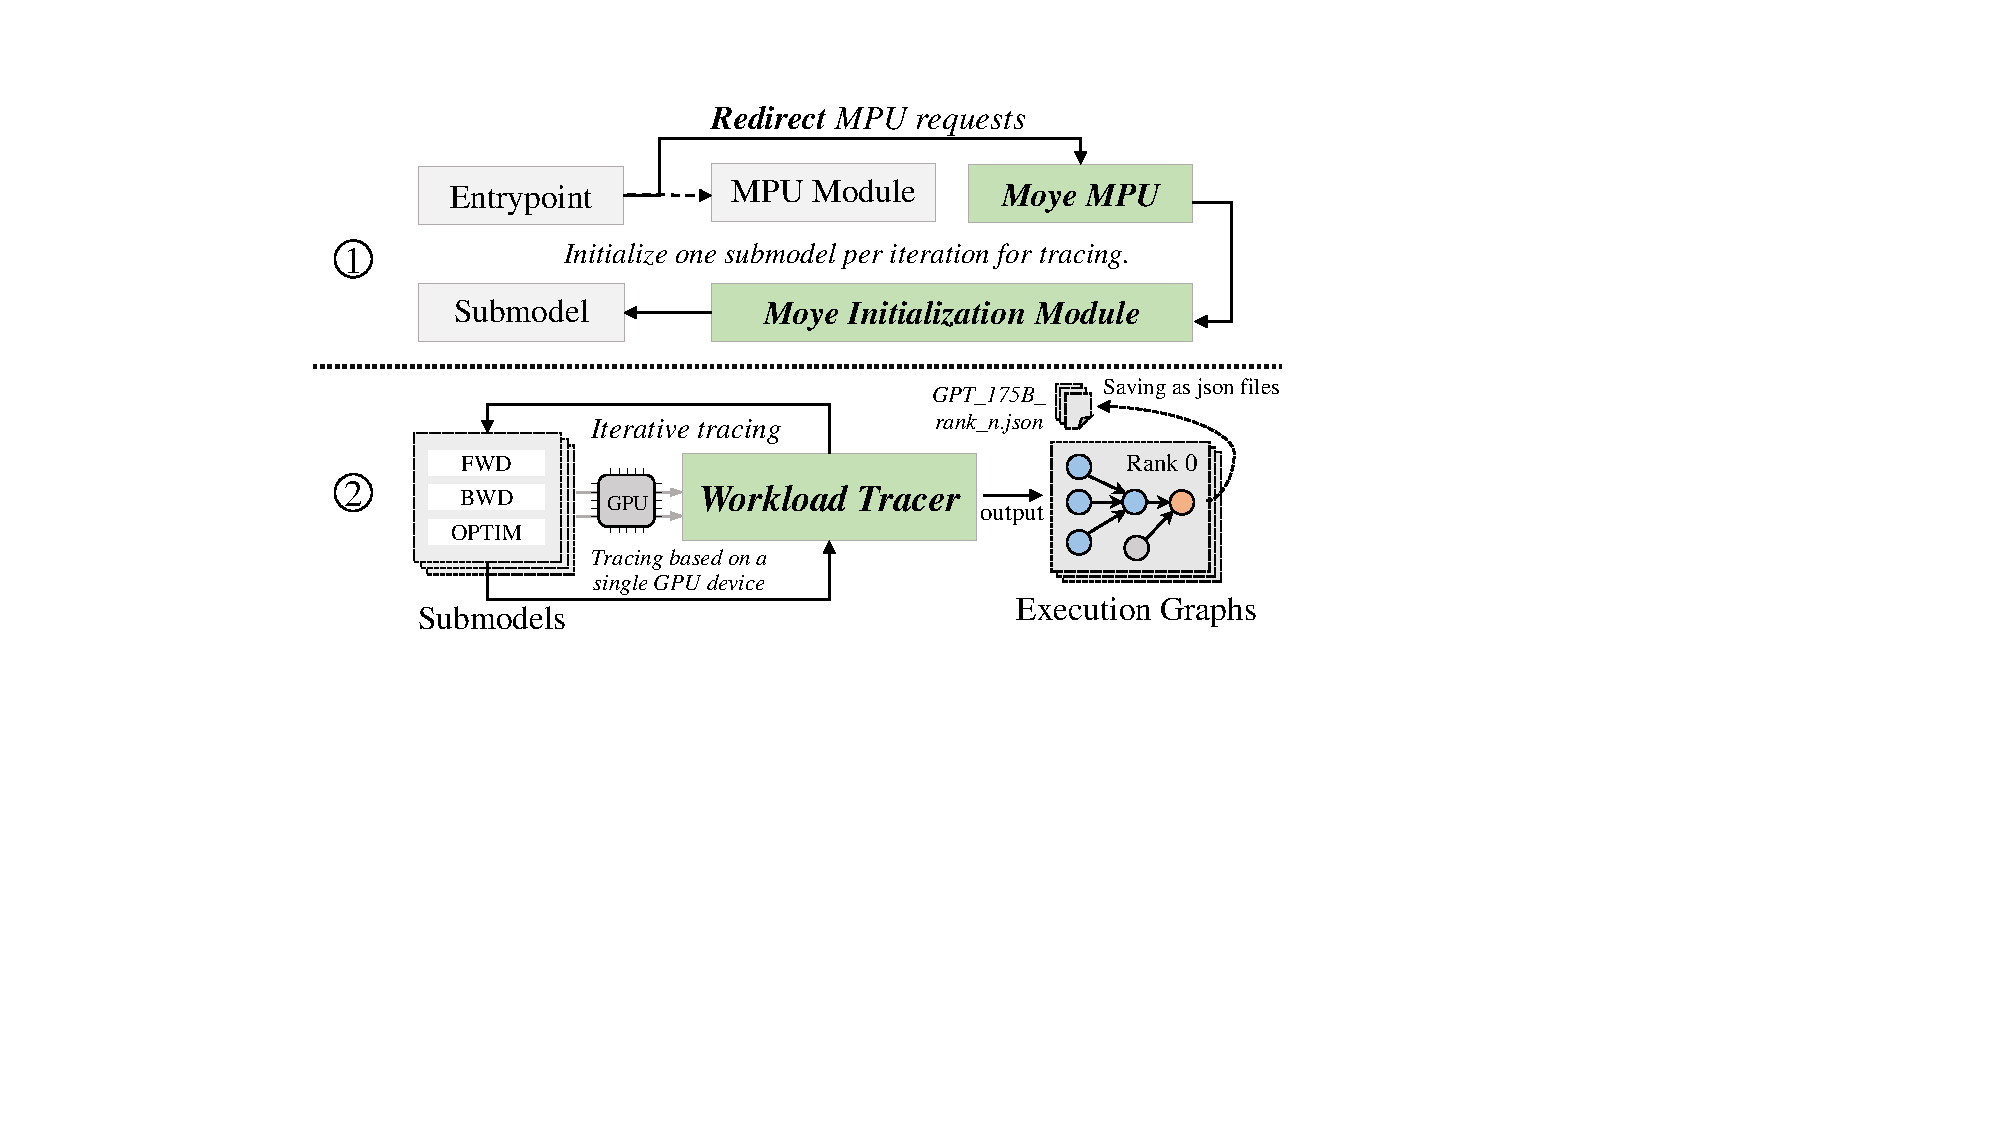
\includegraphics[width=\linewidth]{figures/design/moye_workload_tracer.pdf} 
    % \vspace{-2em}
    \caption{\sys's MPU module and workload tracer.} 
    \label{fig:profier} 
    \vspace{-1em}
\end{figure}

Note that after per-rank workload tracing, all collective communication \ops on the per-node execution graph are placeholders without any running time.
The job of \sys's \cm and \va is precisely to estimate and refine the communication times, respectively, in the next phase.
% In 3D parallelism, generating the complete workload for a training job involves three key steps. First, the model parameters are parsed (e.g., model structure, parallel training settings). Then, the model parallel unit (MPU) module uses these parameters to determine the submodel structure for each rank (typically, one rank per GPU). Finally, each rank initializes its submodel, moving it to the appropriate GPU. \sys allows users to pass simulation-specific parameters to initialize a simulated training environment within the current training framework. 

% When the simulation environment is activated, calls to the standard MPU are redirected to \sys's MPU module, which replaces the original parameters with simulated ones (e.g., number of GPUs, PP and TP configurations). As a result, \sys can determine the submodel to be deployed on each rank. However, at this point, \sys cannot directly execute forward or backward passes on these submodels, as their module implementations contain communication operations (e.g., all-reduce in TP). By restricting the visible GPUs to a single device through \sys's MPU module, \sys bypasses communication dependencies, enabling accurate execution of the workload on a single GPU. To ensure all ranks' workloads are properly initialized, \sys performs this initialization iteratively, simulating distributed behavior without requiring physical cluster resources.

% Unlike previous tools, which often segment the graph when encountering communication operators, \sys treats communication operations as placeholders within the \wg, recording their meta-information (e.g., group associations, message sizes, etc.) and positions within the graph. These placeholders are later replaced with actual runtime estimates during the communication simulation phase~(§X) \jz{(fix this)}. Additionally, \sys provides a lightweight context manager that allows users to adjust the granularity and scope of the trace. For instance, in Megatron-LM's 3D parallelism mode, \sys allows multiple computation operations to be merged into a single operation for simplification. 





\subsection{Timeline Composing } 
\label{subsec:workload_replay}
% \jz{(Workload replay is performed after communication estimator. So this part should be moved to the back?)}

\noindent Before presenting the communication estimation and validation, we discuss how \sys obtains the end-to-end training step time by composing the global timeline with the per-rank workloads obtained above.
%  \ma simulates the end-to-end training process by replaying the per-rank execution graphs.  

Assuming all communication running times are known, \sys's \ma can recover the training process by replaying the per-rank execution graphs.
%  according to the dependencies encoded within. 
\ma is an event-driven simulator that walks through the per-rank execution graphs and puts all \ops (events) onto the global timelines accordingly, including the computation timeline, communication timeline, and memory copy (memcpy) timeline. 
As shown in Figure~\ref{fig:timeline}, a critical piece of information missing from the per-rank graphs is dependencies across ranks; for instance the downstream stages in rank $i$ requires activations from the upstream stages in rank $i-1$ before starting the forward computation in PP.
We provide predefined dependencies and matching rules for both inter-stage and intra-stage events for common parallelism strategies, such as 1F1B.
To enhance flexibility, this module is exposed as an API, allowing users to input new dependencies and matching rules for custom strategies.

While it is possible to strictly replay dependencies through every synchronization across all communication groups, this would significantly increase the timeline construction overhead. 
Instead, \sys leverages workload characteristics to selectively relax synchronization in order to accelerate simulation. 
For instance, in dense models, since each TP rank processes identical sequence lengths, the computation is inherently balanced, allowing us to ignore synchronization delays in TP all-reduce. 
For MoE models, however, load imbalance in the FFN layers requires \sys to preserve the full dependency logic to ensure correctness. In MoE workloads, this conservative treatment is necessary because expert dispatch, expert compute, and expert combine are no longer uniform across ranks: routing imbalance can make a subset of EP ranks the critical-path stragglers. Relaxing these dependencies would therefore bias both tail latency and end-to-end step time.

% Events are mapped to the corresponding timeline based on their attributes.


\begin{figure}[t] 
    \centering 
    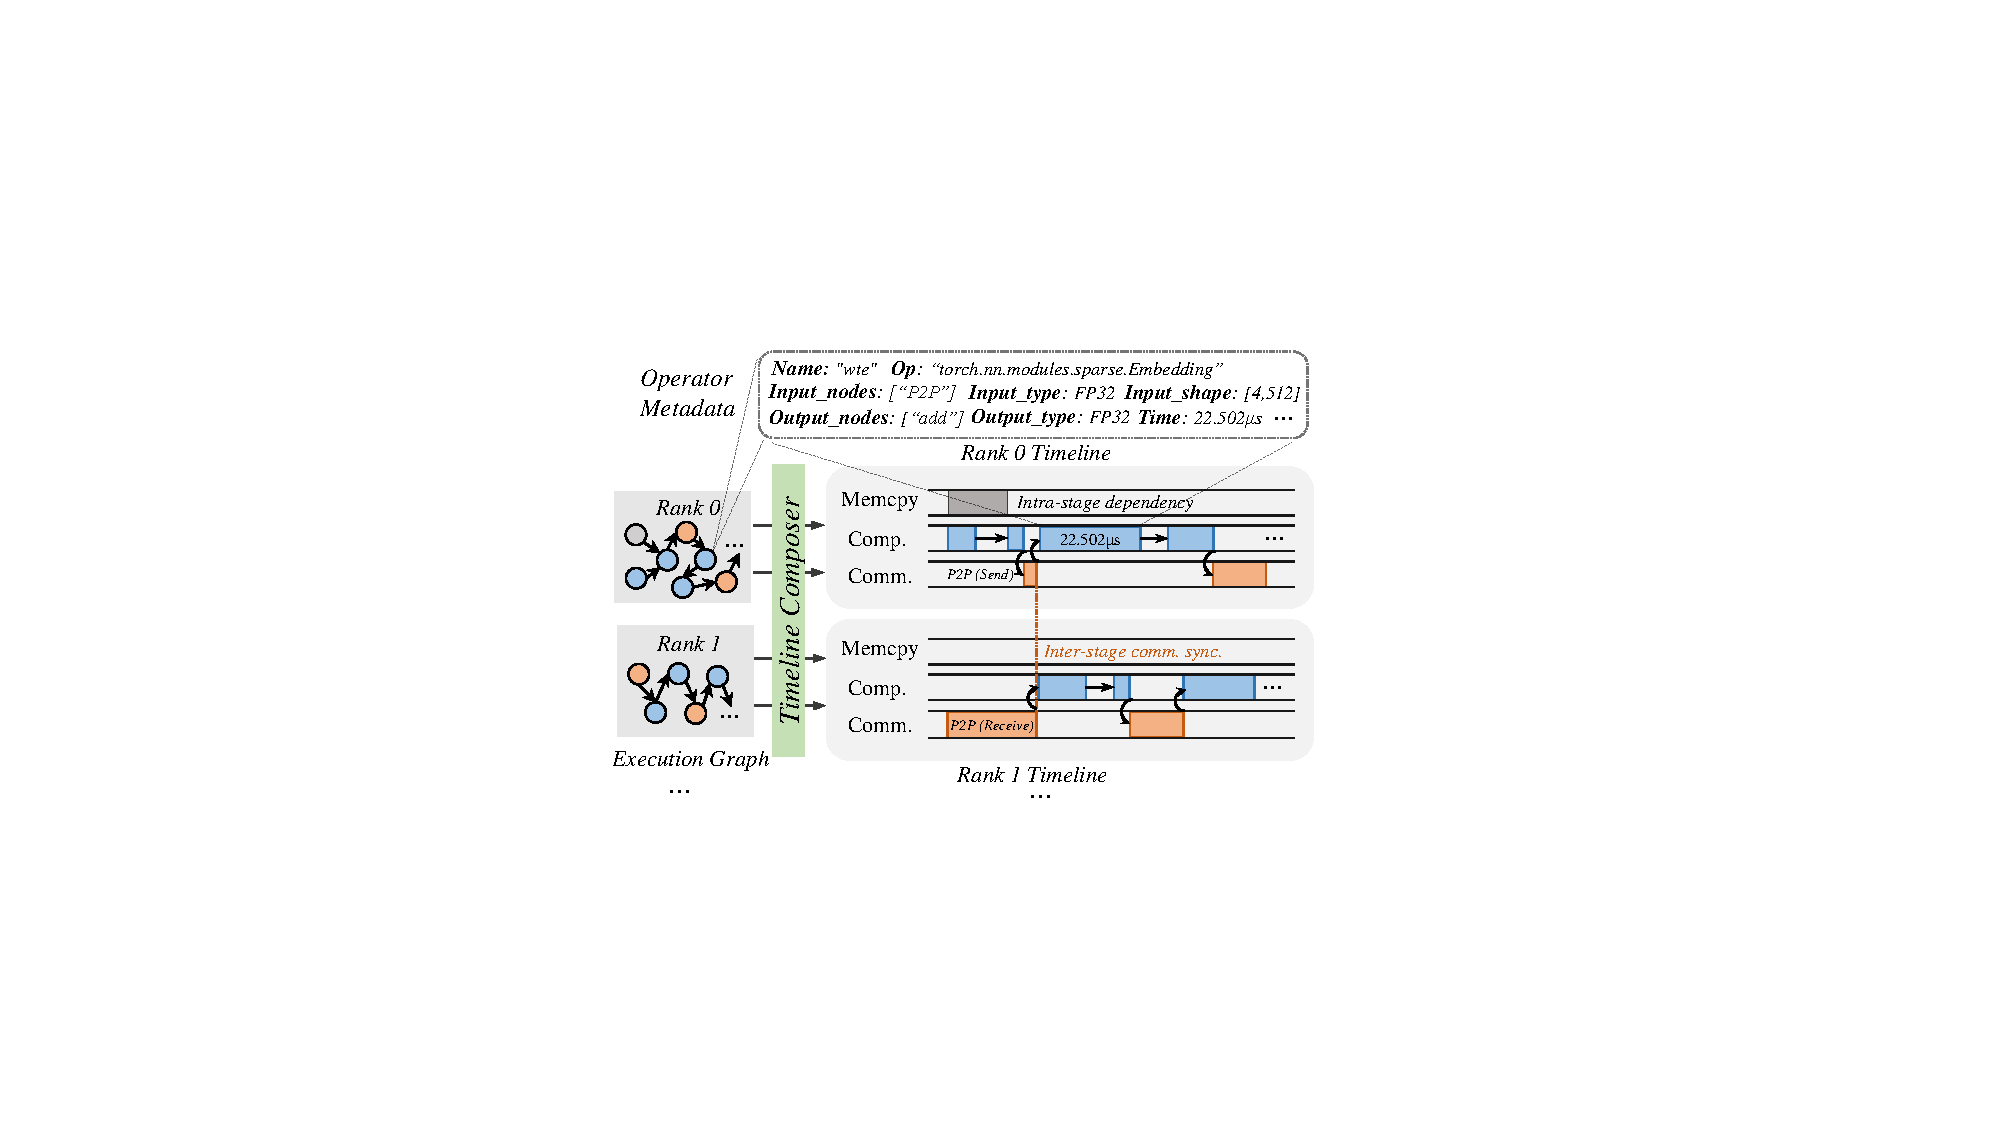
\includegraphics[width=\linewidth]{figures/design/moye_timeline.pdf} 
    \vspace{-1.5em}
    \caption{Illustration of how \sys schedules operations in the execution graph to timelines across ranks.} 
    \label{fig:timeline} 
    \vspace{-1em}
\end{figure}

% \noindent \textbf{Dependencies managing.}
% Additionally, \sys includes predefined dependencies and matching rules for both inter-stage and intra-stage events. For example, in a 1F1B scheduling strategy, downstream stages wait for activation data from upstream stages before starting forward computation. 
